\documentclass[11pt]{article}
\usepackage[a4paper,margin=1in]{geometry}
\usepackage{amsmath,amssymb,amsthm}
\usepackage{tikz}
\usepackage{xcolor}
\usepackage[hidelinks]{hyperref}
\hypersetup{pdftitle={Prime squares and half-turns},pdfauthor={Vamshi Jandhyala}}
\setlength{\parskip}{0.4em}
\setlength{\parindent}{0pt}

\newtheorem{theorem}{Theorem}
\newtheorem{lemma}{Lemma}
\theoremstyle{remark}
\newtheorem*{remark}{Remark}

\definecolor{inkblue}{RGB}{40,76,105}
\definecolor{softblue}{RGB}{226,235,243}
\definecolor{rust}{RGB}{153,70,45}

\newcommand{\Z}{\mathbb{Z}}

\title{Prime squares and half-turns}
\author{Vamshi Jandhyala}
\date{}

\begin{document}
\maketitle
\vspace{-2em}

\begin{abstract}
Can a $p\times p$ square, $p$ prime, be cut into $p$ congruent pieces of $p$ unit cells other than $1\times p$
bars? The question is open when the pieces may be turned and reflected freely. We show that the answer is no
when every piece is a translate of one fixed piece or of its half-turn, for every prime $p$ and without
assuming the piece is connected; for odd $p$ the half-turn may be replaced by any one fixed reflection of the
square. The proof encodes the tiling as an identity between Laurent polynomials and counts orientations by
evaluating a divisibility at $(1,1)$. The algebraic core is checked in the Lean proof assistant.
\end{abstract}

\section{The question}

A $p$-omino is a connected set of $p$ unit cells. JetfiRex asked on Mathematics Stack Exchange and on
MathOverflow~\cite{MSE,MO} whether a $p\times p$ square, with $p$ prime, can be cut into $p$ congruent
$p$-ominoes in any way other than into $p$ straight bars. Stop and try $p=3$ before reading on: the only
other tromino is the L, and three L's cannot fill a $3\times3$ square (the corner cells force it quickly).

\begin{figure}[ht]
\centering
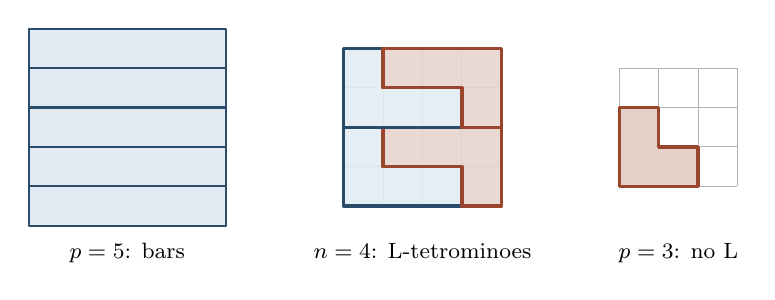
\begin{tikzpicture}[scale=0.5,line join=round]
  % five bars of length five
  \begin{scope}
    \foreach \r in {0,...,4}{\filldraw[fill=softblue,draw=inkblue,thick] (0,\r) rectangle (5,\r+1);}
    \node[below,font=\footnotesize] at (2.5,-0.2) {$p=5$: bars};
  \end{scope}
  % 4 x 4 by four L-tetrominoes, two related by a half-turn in each 2 x 4 half
  \begin{scope}[shift={(8,0.5)}]
    \draw[gray!40,thin] (0,0) grid (4,4);
    \foreach \dy in {0,2}{
      \filldraw[fill=softblue,fill opacity=0.85,draw=inkblue,very thick] (0,\dy) -- (3,\dy) -- (3,\dy+1) -- (1,\dy+1) -- (1,\dy+2) -- (0,\dy+2) -- cycle;
      \filldraw[fill=rust!25,fill opacity=0.85,draw=rust,very thick] (3,\dy) -- (4,\dy) -- (4,\dy+2) -- (1,\dy+2) -- (1,\dy+1) -- (3,\dy+1) -- cycle;
    }
    \node[below,font=\footnotesize] at (2,-0.7) {$n=4$: L-tetrominoes};
  \end{scope}
  % the L-tromino cannot tile 3 x 3
  \begin{scope}[shift={(15,1)}]
    \draw[gray!60] (0,0) grid (3,3);
    \filldraw[fill=rust!25,draw=rust,very thick] (0,0) -- (2,0) -- (2,1) -- (1,1) -- (1,2) -- (0,2) -- cycle;
    \node[below,font=\footnotesize] at (1.5,-1.2) {$p=3$: no L};
  \end{scope}
\end{tikzpicture}

\caption{Left: the bar tiling, which works for every $n$. Middle: for $n=4$ the L-tetromino tiles the square,
and each $2\times4$ half is an L together with its half-turn, so composite sizes have other tilings even
with only translations and half-turns. Right: the L-tromino, which cannot tile the $3\times3$ square.}
\label{fig:tilings}
\end{figure}

The answer depends on primality (Figure~\ref{fig:tilings}). An exhaustive search, allowing all eight
orientations, finds only bars for every prime $p\le 13$; for composite $n\le14$ there are always other
tilings. The question is a discrete case of an older one. Danzer conjectured that a square cannot be cut
into five congruent polygons, convex or not, other than rectangles, and that conjecture is still
open~\cite{MRP22}. For convex pieces much more is known: the square cannot be cut into $5$, $7$ or $9$
congruent convex pieces other than rectangles~\cite{YZZ16,MRP22}. Yuan, Zamfirescu and Zamfirescu asked
whether the same holds for every prime number of convex pieces, and Rao, Ren and Wang conjectured it for every
odd number~\cite{RRW20}. A polyomino need not be convex, so none of this
applies. For three pieces Maltby classified all ways to cut a rectangle into three congruent topological
discs~\cite{Mal94}, which settles $p=3$.

This note proves the question in a restricted form, in which the pieces may be moved by translations and
half-turns but not by quarter-turns or reflections.

\begin{theorem}\label{thm:half}
Let $p$ be prime and let $P$ be a set of $p$ cells, not necessarily connected. If the $p\times p$ square is
tiled by $p$ copies of $P$, each a translate of $P$ or of its half-turn, then $P$ is a straight bar.
\end{theorem}

\begin{theorem}\label{thm:refl}
Let $p$ be an odd prime and let $\tau$ be one of the four reflections of the square. If the square is tiled by
$p$ copies of a $p$-cell set $P$, each a translate of $P$ or of $\tau(P)$, then $P$ is a straight bar.
\end{theorem}

With translations alone the conclusion is close to known results: if translates of a set of prime size tile
$\Z^n$, then some lattice of its translates tiles $\Z^n$ too, a theorem of Szegedy~\cite{Sze98} to which
Horak and Kim gave a polynomial proof~\cite{HK16}. We do not claim the translation-only case as new. The point here is that a second
orientation can be allowed, and the proof is a page of algebra.

\section{Cells as monomials}

Let $p$ be odd for now and put $m=(p-1)/2$. Index the cells of the board by their centres $(i,j)$ with
$-m\le i,j\le m$, and give each cell the monomial $x^iy^j$. A set of cells becomes the sum of its monomials
(Figure~\ref{fig:encoding}). Exponents may be negative, so we work in the ring
$A=\Z[x,x^{-1},y,y^{-1}]$ of integer Laurent polynomials. Three features of $A$ make it convenient.

\begin{figure}[ht]
\centering
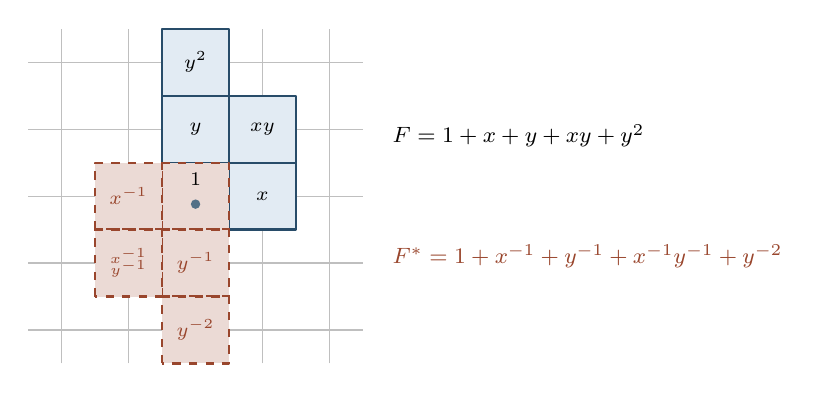
\begin{tikzpicture}[scale=0.85,line join=round]
  % the 5 x 5 board centred at the origin; a P-pentomino and its half-turn
  \draw[gray!50] (-2.5,-2.5) grid (2.5,2.5);
  \foreach \c in {(0,0),(1,0),(0,1),(1,1),(0,2)}{\filldraw[fill=softblue,draw=inkblue,thick] \c ++(-0.5,-0.5) rectangle ++(1,1);}
  \foreach \c in {(0,0),(-1,0),(0,-1),(-1,-1),(0,-2)}{\filldraw[fill=rust!20,draw=rust,thick,dashed] \c ++(-0.5,-0.5) rectangle ++(1,1);}
  \fill[inkblue!80] (0,-0.12) circle (2pt);
  \node[font=\scriptsize] at (1,0) {$x$};
  \node[font=\scriptsize] at (0,1) {$y$};
  \node[font=\scriptsize] at (1,1) {$xy$};
  \node[font=\scriptsize] at (0,2) {$y^2$};
  \node[font=\scriptsize] at (0,0.25) {$1$};
  \node[font=\scriptsize,rust] at (-1,0) {$x^{-1}$};
  \node[font=\scriptsize,rust] at (0,-1) {$y^{-1}$};
  \node[font=\tiny,rust,align=center] at (-1,-1) {$x^{-1}$\\[-2pt]$y^{-1}$};
  \node[font=\scriptsize,rust] at (0,-2) {$y^{-2}$};
  \node[right,font=\footnotesize,align=left] at (2.8,0.9) {$F=1+x+y+xy+y^2$};
  \node[right,font=\footnotesize,align=left,rust] at (2.8,-0.9) {$F^*=1+x^{-1}+y^{-1}+x^{-1}y^{-1}+y^{-2}$};
\end{tikzpicture}

\caption{A P-pentomino (solid) and its half-turn about the centre (dashed), with the monomial of each cell.
The half-turn is the substitution $x\mapsto x^{-1}$, $y\mapsto y^{-1}$.}
\label{fig:encoding}
\end{figure}

\emph{Translations are units.} Moving a set by $(a,b)$ multiplies its polynomial by $x^ay^b$, and the units of
$A$ are exactly the signed monomials $\pm x^ay^b$.

\emph{The half-turn is a ring automorphism.} Write $H^*(x,y)=H(x^{-1},y^{-1})$. This is the half-turn about the
centre of the board, and it respects sums and products. Each reflection of the square is likewise a
substitution ($x\leftrightarrow x^{-1}$, or $y\leftrightarrow y^{-1}$, or $x\leftrightarrow y$, or
$x\leftrightarrow y^{-1}$), hence an automorphism of $A$ that squares to the identity.

\emph{Unique factorisation, and the board's two factors.} The board is
\[
R=x^{-m}y^{-m}\,Q_p(x)\,Q_p(y),\qquad Q_p(t)=1+t+\dots+t^{p-1}.
\]
The ring $A$ is a unique factorisation domain, being a localisation of $\Z[x,y]$. The polynomial $Q_p$ is
irreducible over $\Z$, since $Q_p(t+1)$ is an Eisenstein polynomial at $p$. A prime of $\Z[x]$ stays prime in
$\Z[x][y]$, and a prime of $\Z[x,y]$ that does not divide $xy$ stays prime in the localisation $A$; so $Q_p(x)$
and $Q_p(y)$ are primes of $A$, and up to units they are the only prime factors of $R$. Every map in sight fixes
$R$, and evaluation at $(1,1)$ sends $Q_p(x)$, $Q_p(y)$ and the polynomial $F$ of any $p$-cell set to $p$.

Now suppose the board is tiled as in Theorem~\ref{thm:half}. Let $F$ be the polynomial of $P$, let $U$ be the
sum of the translation monomials used by the copies of $P$, and $V$ the same for the copies of $P^*$. Exact
covering says
\begin{equation}\label{eq:tile}
F\,U+F^*\,V=R .
\end{equation}
Read it as: every cell of the board is covered exactly once, either by a translate of $P$ or by a translate of
its half-turn. If $u$ copies have the first orientation and $v$ the second, evaluation at $(1,1)$ gives
$U(1,1)=u$, $V(1,1)=v$ and $u+v=p$.

\section{Proof}

Everything rests on one question: do $F$ and $F^*$ have a common factor?

\begin{lemma}[a common factor forces a bar]\label{lem:common}
If $Q_p(x)$ divides $F$ in $A$, then $P$ is a horizontal bar; likewise for $Q_p(y)$ and a vertical bar.
\end{lemma}

\begin{proof}
Translate $P$ so that its smallest $x$- and $y$-exponents are $0$; then $F\in\Z[x,y]$ has degree at most $p-1$
in $x$, since a copy of $P$ fits in the board. Clearing denominators in $F=Q_p(x)\,G$ gives
$x^ay^bF=Q_p(x)\,G_0$ with $G_0\in\Z[x,y]$. The prime $Q_p(x)$ of $\Z[x,y]$ divides neither $x$ nor $y$, so it
divides $F$ in $\Z[x,y]$, and therefore divides each row $F_k(x)$, the coefficient of $y^k$ in $F$. A row has
degree at most $p-1$ and coefficients $0$ or $1$; a multiple of $Q_p(x)$ of that degree is $c\,Q_p(x)$ with
$c$ an integer, and $c$ is the constant term, so each row is $0$ or $Q_p(x)$: empty, or a full row of $p$
cells. As $P$ has $p$ cells, exactly one row is full.
\end{proof}

\begin{proof}[Proof of Theorem~\ref{thm:half} for odd $p$]
Suppose first that $F$ and $F^*$ have a common factor that is not a unit. By~\eqref{eq:tile} it divides $R$, so
one of the primes $Q_p(x)$, $Q_p(y)$ divides it, and hence divides $F$; Lemma~\ref{lem:common} gives a bar.

Otherwise $F$ and $F^*$ are coprime. Apply ${}^*$ to~\eqref{eq:tile}; as $R^*=R$ and ${}^{**}$ is the identity,
$F^*U^*+F\,V^*=R$. Subtracting this from~\eqref{eq:tile},
\[
F\,(U-V^*)=F^*\,(U^*-V).
\]
Since $F$ is coprime to $F^*$, it divides $U^*-V$: there is $H\in A$ with $U^*-V=F\,H$. Evaluate at $(1,1)$.
The left side becomes $u-v$, and the right side $p\,H(1,1)$, an integer multiple of $p$. Together with
$u+v=p$ this says $p$ divides $2u$; as $p$ is odd, $u=0$ or $u=p$. So all the copies have the same
orientation, and~\eqref{eq:tile} reads $F\,U=R$ or $F^*V=R$. In the second case apply ${}^*$. Either way $F$
divides $R$. As $F(1,1)=p$ is not $\pm1$, $F$ is not a unit, so one of the primes $Q_p(x)$, $Q_p(y)$ divides $F$, and Lemma~\ref{lem:common} gives a bar.
\end{proof}

\emph{The case $p=2$.} Any two cells are symmetric about their midpoint, so the half-turn of $P$ is a translate
of $P$ and the tiling uses translations only: $F\,U=R$ with $R=(1+x)(1+y)$, indexing cells from $0$. As
$F(1,1)=2$, $F$ is not a unit, so $1+x$ or $1+y$ divides $F$, and Lemma~\ref{lem:common}, whose proof never
used that $p$ is odd, gives a domino.

\begin{proof}[Proof of Theorem~\ref{thm:refl}]
Replace the half-turn by the substitution of the chosen reflection. Nothing in the proof used more than three
facts about ${}^*$: it is a ring automorphism of $A$ of order two, it fixes $R$, and it commutes with
evaluation at $(1,1)$. All three hold for each reflection.
\end{proof}

Oddness matters in Theorem~\ref{thm:refl}. For $p=2$ the two cells on a diagonal of the $2\times2$ square,
together with their mirror image in a vertical line, tile it. The orientation count is where the proof breaks:
$p=2$ divides $2u$ for every $u$.

\begin{remark}
The argument stops at quarter-turns. If $\rho$ is a quarter-turn, applying $\rho$ to $F\,U+\rho(F)\,V=R$
produces $\rho(F)\rho(U)+\rho^2(F)\rho(V)=R$, which involves a third tile polynomial $\rho^2(F)$, and the
subtraction no longer isolates two coprime factors. Two different reflections fail in the same way. The full
question needs a further idea.
\end{remark}

\paragraph{Verification.} Lemma~\ref{lem:common} in polynomial form and the orientation argument are checked in
Lean~4 with Mathlib~\cite{mathlib}, using only the standard axioms. The orientation argument is formalised once
for any unique factorisation domain with an involutive automorphism ${}^*$ fixing $R=q_1q_2$ ($q_1,q_2$ prime)
and an evaluation to $\Z$ fixed by ${}^*$, so it covers Theorems~\ref{thm:half} and~\ref{thm:refl} together.
Quoted rather than formalised: that $A$ is a unique factorisation domain in which $Q_p(x)$ and $Q_p(y)$ are
prime, and the passage from a tiling to~\eqref{eq:tile}. A Python program audits each ingredient in exact
arithmetic (cell images under the eight symmetries, the substitutions, the factor obstruction, the quotients
and the orientation counts, with a composite control), and deliberately wrong variants fail it. A C program
searches exhaustively for $n\le14$ with all eight orientations, and an independent program, sharing no code
with the others, enumerates the tilings with translations and one second orientation for small primes,
including disconnected pieces for $p\le5$. Everything is at
\url{https://github.com/jvvk/mathematics/tree/main/prime-squares-half-turns}.

\paragraph{Acknowledgements.} JetfiRex asked the question. Anthropic's Claude (Opus~5.5) was used to find the
argument, write the Lean formalisation and the programs, and draft this text. The author takes
responsibility for the content.

\begin{thebibliography}{9}
\bibitem{MSE} JetfiRex, Is there only one way to dissect a $p\times p$ square into $p$ congruent $p$-ominoes, for
prime $p$?, Mathematics Stack Exchange question 5007342 (5 December 2024),
\url{https://math.stackexchange.com/q/5007342}, accessed 10 October 2026.
\bibitem{MO} JetfiRex, the same question on MathOverflow, question 487157 (4 February 2025),
\url{https://mathoverflow.net/q/487157}, accessed 10 October 2026.
\bibitem{HK16} P.~Horak and D.~Kim, Polynomial method in tilings, arXiv:1603.00051 (2016).
\bibitem{Mal94} S.~J.~Maltby, Trisecting a rectangle, \emph{J. Combin. Theory Ser. A} \textbf{66} (1994) 40--52,
\href{https://doi.org/10.1016/0097-3165(94)90049-3}{doi:10.1016/0097-3165(94)90049-3}.
\bibitem{MRP22} G.~L.~Maldonado and E.~Rold\'an-Pensado, Dissecting the square into seven or nine congruent
parts, \emph{Discrete Math.} \textbf{345} (2022) 112800,
\href{https://doi.org/10.1016/j.disc.2022.112800}{doi:10.1016/j.disc.2022.112800}.
\bibitem{RRW20} H.~Rao, L.~Ren and Y.~Wang, Dissecting a square into congruent polygons, \emph{Discrete Math.
Theor. Comput. Sci.} \textbf{22}:1 (2020) \#21,
\href{https://doi.org/10.23638/DMTCS-22-1-21}{doi:10.23638/DMTCS-22-1-21}.
\bibitem{Sze98} M.~Szegedy, Algorithms to tile the infinite grid with finite clusters, in \emph{Proceedings of
the 39th Annual Symposium on Foundations of Computer Science}, IEEE, 1998, 137--145,
\href{https://doi.org/10.1109/SFCS.1998.743437}{doi:10.1109/SFCS.1998.743437}.
\bibitem{YZZ16} L.~Yuan, C.~T.~Zamfirescu and T.~I.~Zamfirescu, Dissecting the square into five congruent parts,
\emph{Discrete Math.} \textbf{339} (2016) 288--298,
\href{https://doi.org/10.1016/j.disc.2015.08.009}{doi:10.1016/j.disc.2015.08.009}.
\bibitem{mathlib} The mathlib Community, The Lean mathematical library, in \emph{Proceedings of the 9th ACM
SIGPLAN International Conference on Certified Programs and Proofs (CPP 2020)}, 367--381,
\href{https://doi.org/10.1145/3372885.3373824}{doi:10.1145/3372885.3373824}.
\end{thebibliography}

\bigskip
\noindent Vamshi Jandhyala, London, UK.

\end{document}
